\subsubsection{Scope}

\begin{figure}[H]
	\centering
	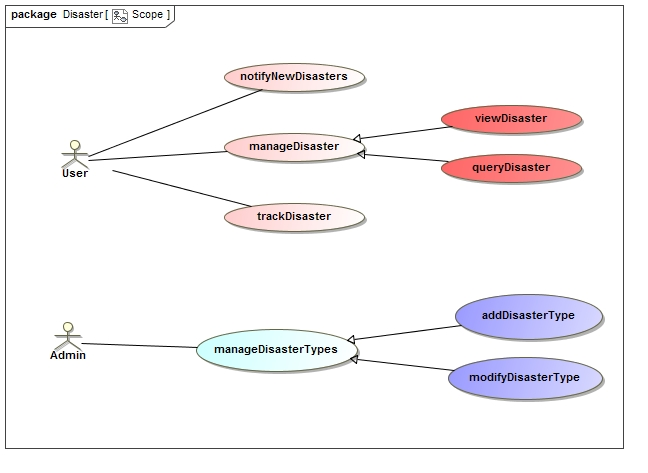
\includegraphics[scale=0.77]{../images/funcReq/DisasterScope.jpg}
	\caption{The scope of functionality required from the disaster module \label{overflow}}
\end{figure}

Admin can add and/or modify the different kinds of disaster types that are required whilst users are able to track and manage disasters as well as get notifications for new disasters. 

\subsubsection{addDisasterType}

Adding a disaster type requires that the user has admin rights and that there should not be a disaster type of the same name as the one being added that exists. If the user is admin and the disaster type being added is unique then a new disaster type will be added to the system. Below are the service contract, activity diagram and functional requirements diagram for addDisasterType.

\begin{figure}[H]
	\centering
	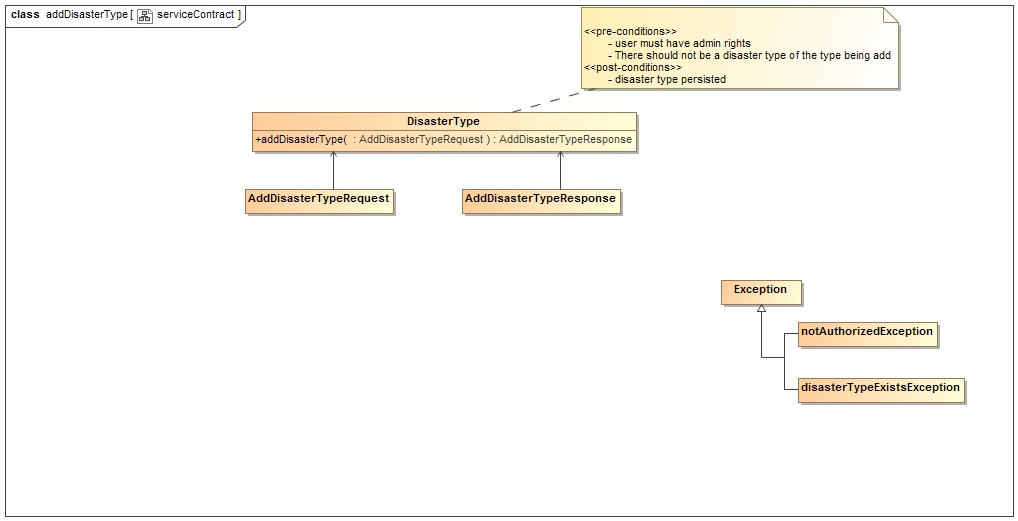
\includegraphics[width=1.0\textwidth]{../images/addDisasterTypeServiceContract.jpg}
	\caption{The service contract for addDisasterType \label{overflow}}
\end{figure}

\begin{figure}[H]
	\centering
	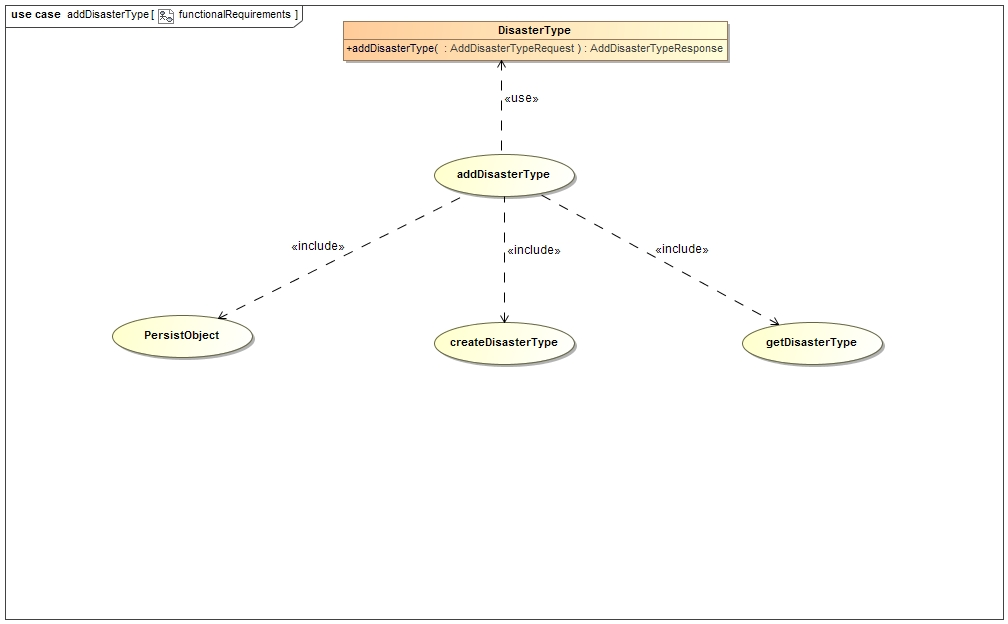
\includegraphics[width=1.0\textwidth]{../images/AddDisasterTypeFunctionalRequirements.jpg}
	\caption{The functional requirements diagram for addDisasterType \label{overflow}}
\end{figure}

\begin{figure}[H]
	\centering
	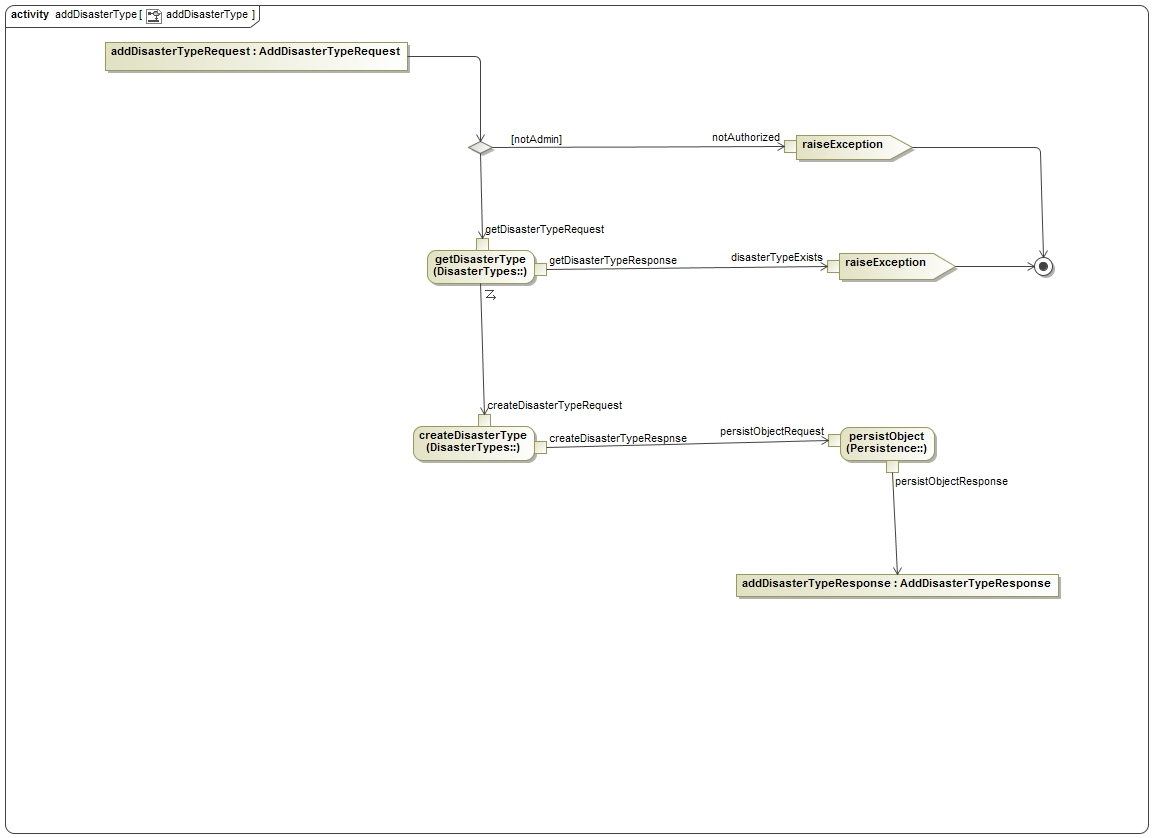
\includegraphics[width=1.0\textwidth]{../images/addDisasterTypeActivityDiagram.jpg}
	\caption{The activity diagram for addDisasterType \label{overflow}}
\end{figure}

\subsubsection{viewDisaster}

A user can view disasters by going on to the disasters tab on the system and being able to view all the active disasters occurring throughout the world. Below are the service contract, activity diagram and functional requirements diagram for viewDisaster.

\begin{figure}[H]
	\centering
	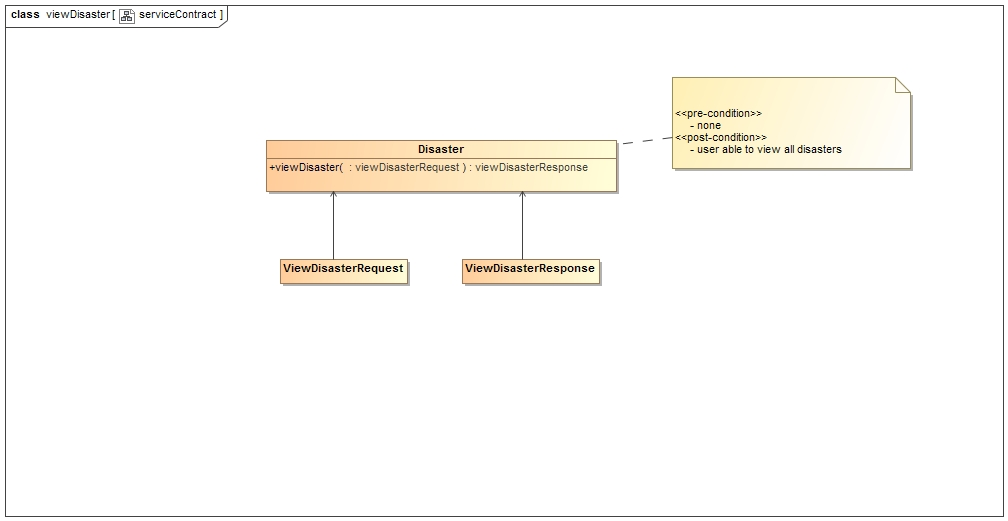
\includegraphics[width=1.0\textwidth]{../images/viewDisasterServiceContract.jpg}
	\caption{The service contract for viewDisaster \label{overflow}}
\end{figure}

\begin{figure}[H]
	\centering
	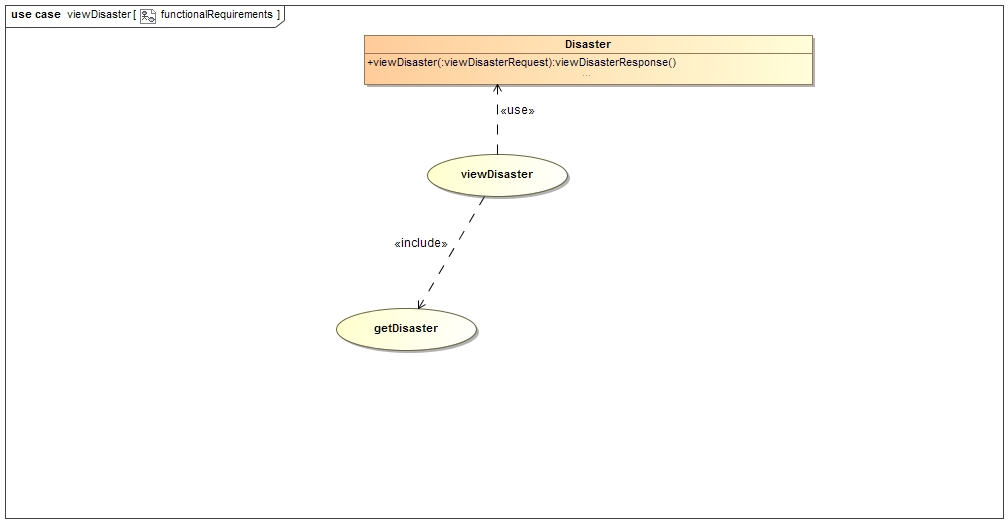
\includegraphics[width=1.0\textwidth]{../images/viewDisasterFunctionalRequirements.jpg}
	\caption{The functional requirements diagram for viewDisaster \label{overflow}}
\end{figure}

\begin{figure}[H]
	\centering
	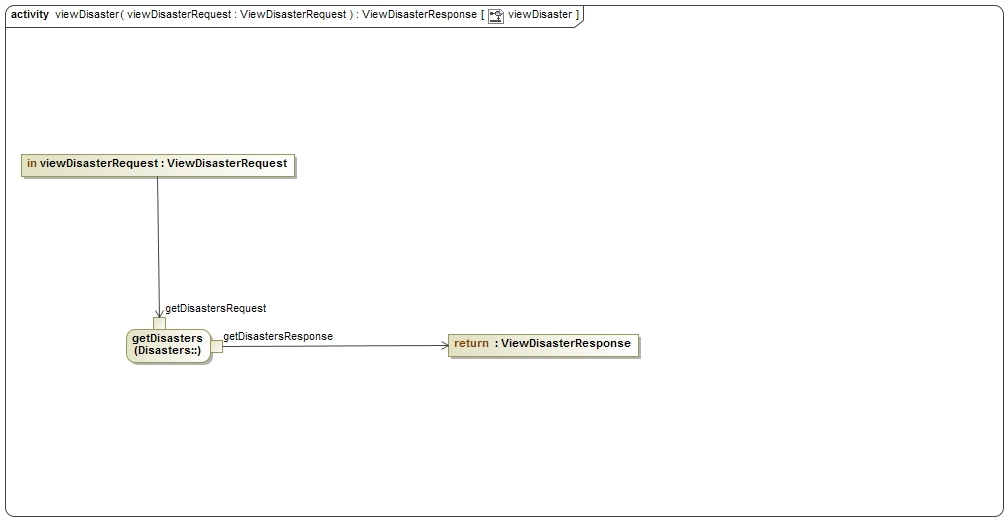
\includegraphics[width=1.0\textwidth]{../images/viewDisasterActivityDiagram.jpg}
	\caption{The activity diagram for viewDisaster \label{overflow}}
\end{figure}

\subsubsection{queryDisaster}

The user will be able to query the system for specific disasters, by entering search criteria so that only data matching the specified criteria is returned to the user. Below are the service contract, activity diagram and functional requirements diagram for queryDisaster.

 \begin{figure}[H]
	\centering
	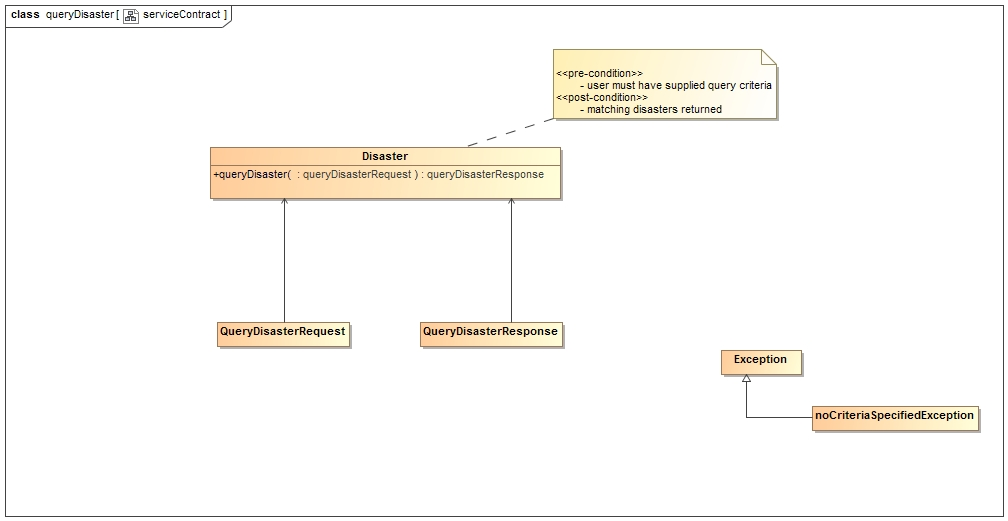
\includegraphics[width=1.0\textwidth]{../images/queryDisasterServiceContract.jpg}
	\caption{The service contract for queryDisaster \label{overflow}}
\end{figure}

\begin{figure}[H]
	\centering
	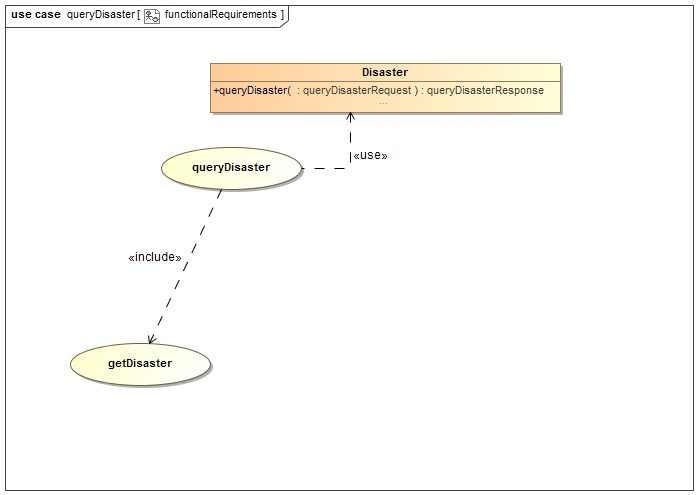
\includegraphics[width=1.0\textwidth]{../images/queryDisasterFunctionalRequirements.jpg}
	\caption{The functional requirements diagram for queryDisaster \label{overflow}}
\end{figure}

\begin{figure}[H]
	\centering
	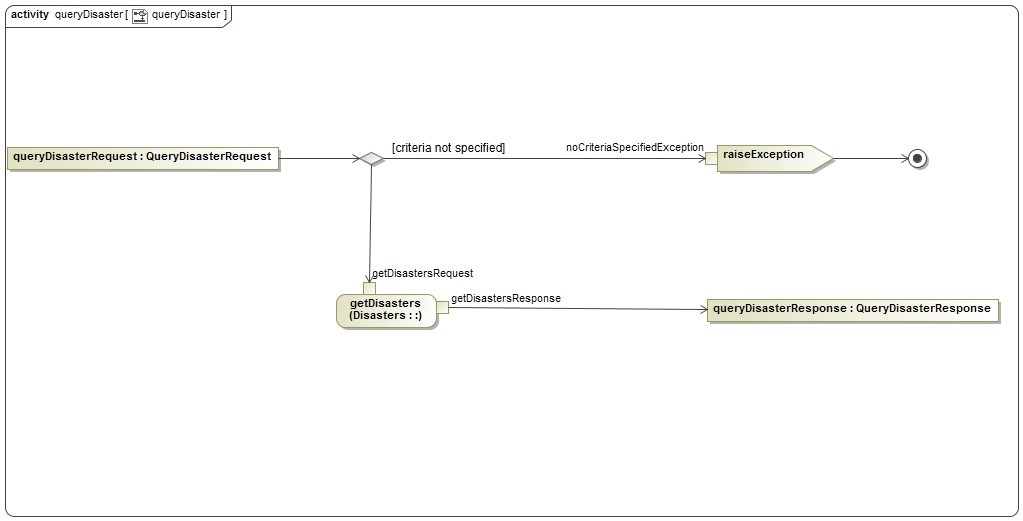
\includegraphics[width=1.0\textwidth]{../images/queryDisasterActivityDiagram.jpg}
	\caption{The activity diagram for queryDisaster \label{overflow}}
\end{figure} 

\subsubsection{hideDisaster}
\subsubsection {trackDisaster}
\subsubsection{notifyNewDisaster}
\subsubsection{modifyDisasterType}
\subsubsection{authenticate}
